\documentclass{article}
\usepackage[utf8]{inputenc}
\usepackage{graphicx}
\usepackage{wrapfig}
\usepackage{array}
\usepackage{siunitx}
\usepackage{xcolor}
\usepackage{multicol}
\usepackage{amssymb}
\usepackage{hyperref}
\setlength{\columnseprule}{1pt}

\title{Speed Control of a DC motor by Armature Voltage Control \\ Lab Project Report \\ ELP100}
\author{Yash Agarwal \\ 2021EE10638 \\ Group 29}
\date{June 22, 2022}

\begin{document}
\pagecolor{yellow!15}
\maketitle
\vspace{15px}
\tableofcontents
\newcolumntype{V}{>{\centering\arraybackslash} m{.4\linewidth} }
\newpage
\section{Aim}
Control the speed of the motor using armature voltage control method. Demonstrate motor running at (i) the rated speed (ii) half the rated speed.

\section{Apparatus}
\begin{enumerate}
\item 555 Timer and variable resistance
\item Capacitors and diodes
\item DSO, wires and power supply
\item BJT
\item Motor

\end{enumerate}

\section{Theory}
\begin{wrapfigure}{R}{0.35\textwidth}
    \fcolorbox{black}{white}{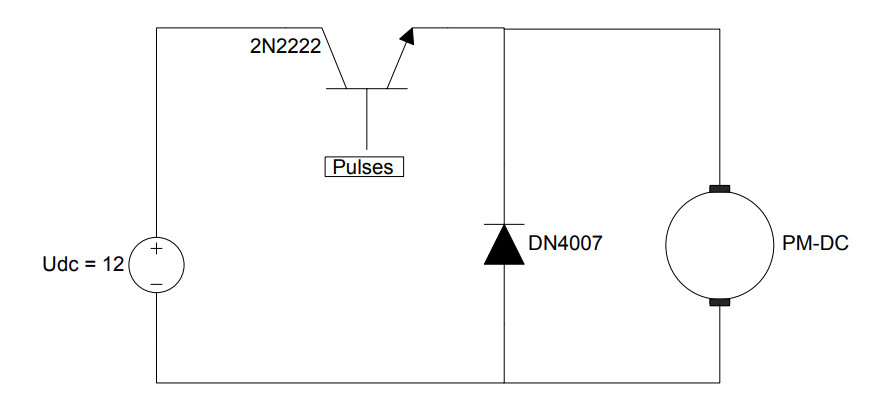
\includegraphics[width=0.35\textwidth]{Screenshot 2022-06-22 163205.png}}
\end{wrapfigure}

PWM (Pulse Width Modulation) is a method through which we can generate variable voltage by turning on and off the power that’s going to the electronic device at a fast rate. The average voltage depends on the duty cycle of the signal, or the amount of time the signal is ON versus the amount of time the signal is OFF in a single period of time.

The 555 Timer is capable of generating PWM signal when set up in an astable mode.
When the output is HIGH when the capacitor C1 is charging through the resistors R1 and R2.
On the other hand, the output of the IC is LOW when the capacitor C1 is discharging but only through the resistor R2.
So we can notice that if we change the values of any of these three components we will get different ON and OFF times, or different duty cycle of the square wave output signal.
The control pin of the 555 Timer is not used but it’s connected to a 10nF capacitor in order to eliminate any external noise from that terminal. The reset, pin number 4, is active low so therefore it is connected to VCC in order to prevent any unwanted reset of the output.
The output of the 555 timer can sink or source a current of 200mA to the load. So if the motor that we want to control exceeds this rating we need to use a transistor or a MOSFET for driving the motor. We used a (TIP122) Darlington transistor which can handle a current up to 5A.
For preventing any voltage spikes produced by the motor we need to use a freewheeling diode which is connected in parallel with the motor.

\section{Circuit Diagram}
\vspace{5px}
\begin{center}
\fcolorbox{black}{white}{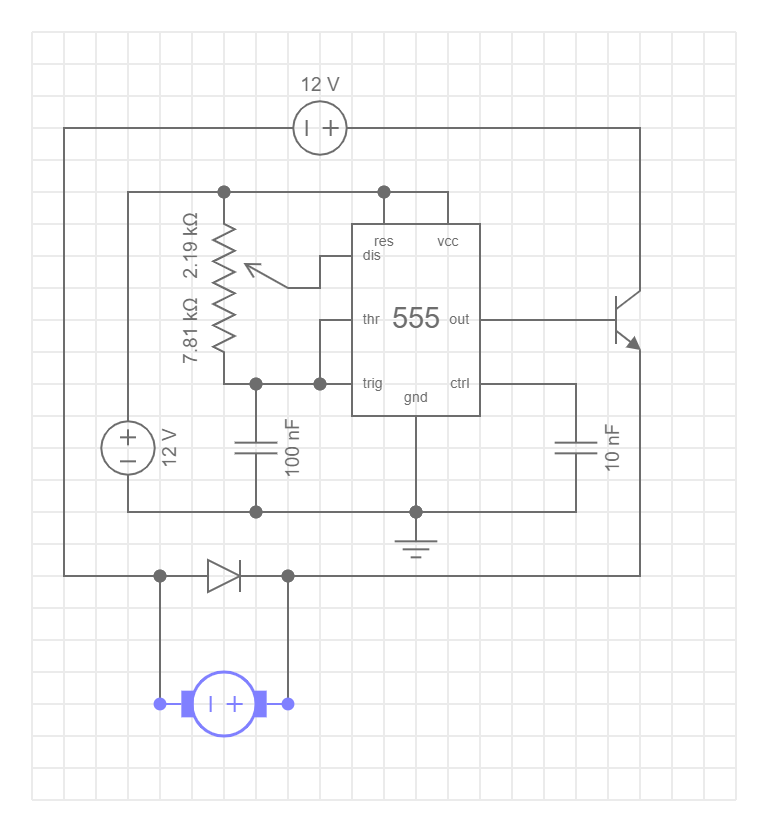
\includegraphics[width=1\columnwidth]{circuit (1).png}}
\end{center}
\vspace{20px}

\section{Breadboard Setup}
\vspace{5px}
\begin{center}
\fcolorbox{black}{white}{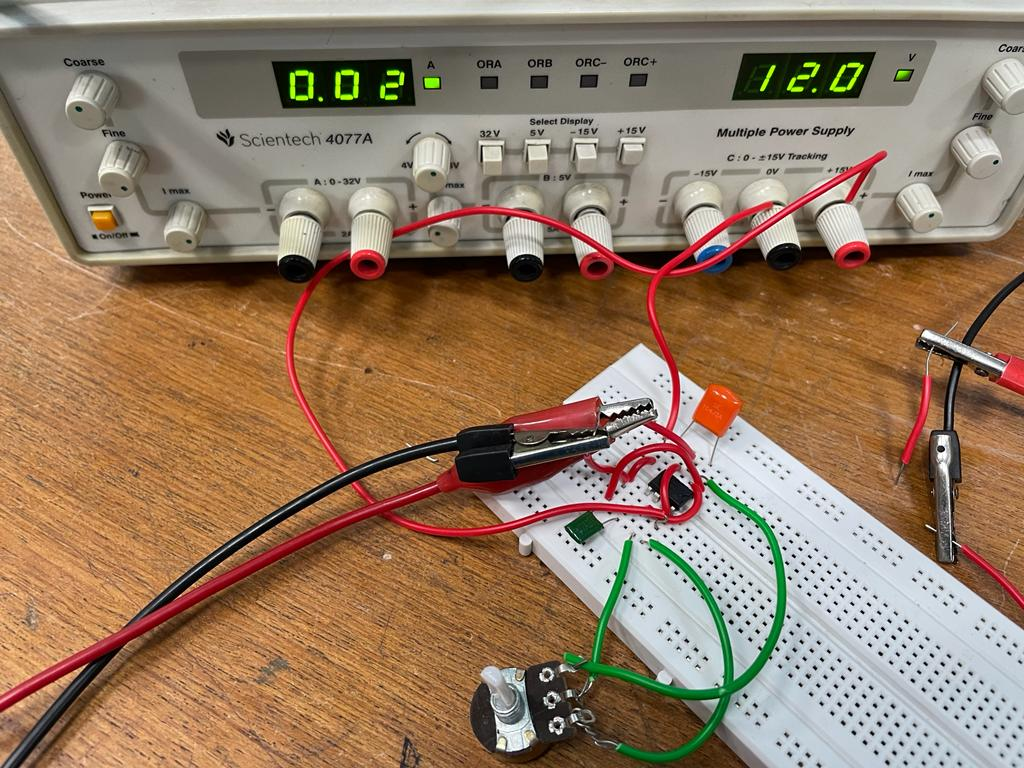
\includegraphics[width=1\columnwidth, height=200px]{WhatsApp Image 2022-06-22 at 12.34.08 PM (6).jpeg}} \\ \vspace{5px}
Control Circuit\\

\vspace{20px}

\hline

\vspace{20px}
Power Circuit\\
\vspace{5px}
\fcolorbox{black}{white}{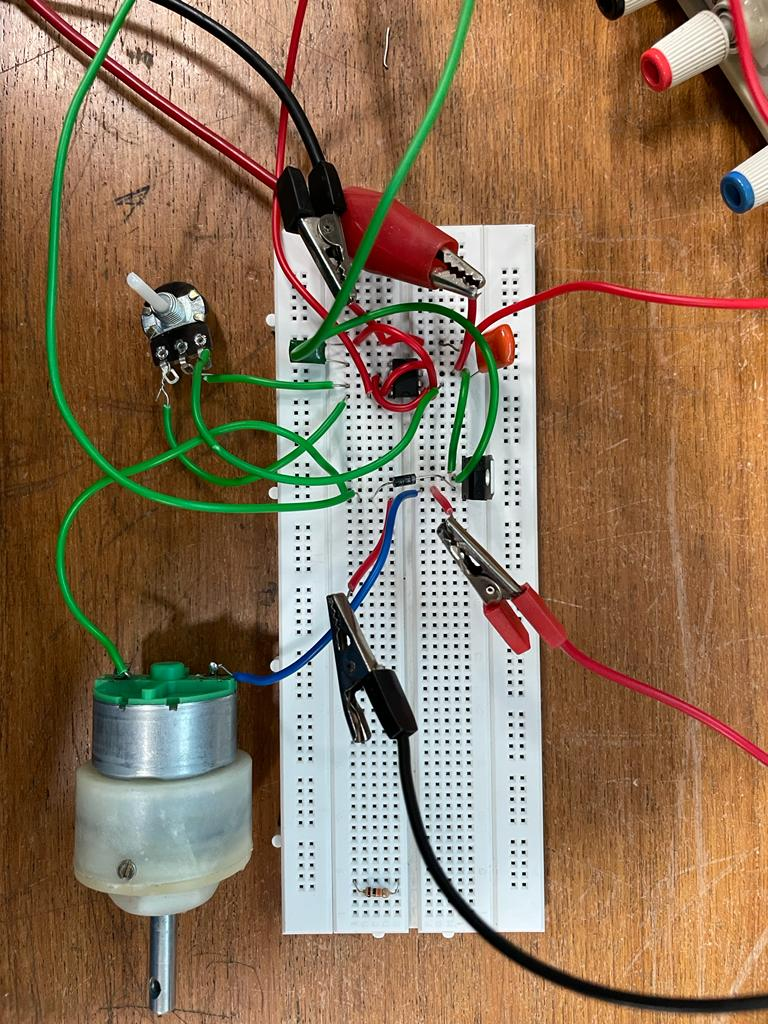
\includegraphics[angle=90,width=1\columnwidth, height=200px]{WhatsApp Image 2022-06-22 at 12.34.08 PM.jpeg}} \\
\end{center}

\newpage

\section{DSO Images}
\vspace{5px}
\subsection{Control Circuit}
\begin{multicols}{2}
\begin{center}
\fcolorbox{black}{white}{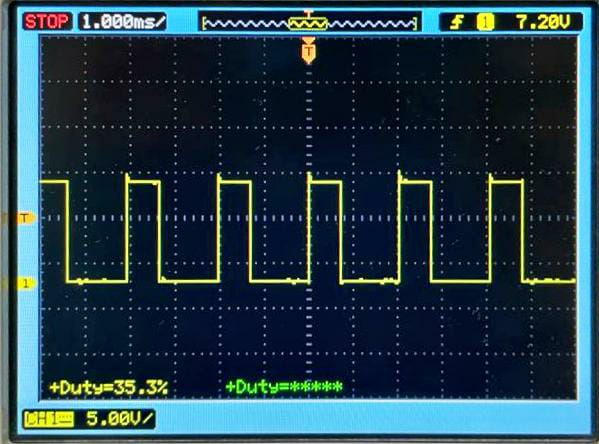
\includegraphics[width=0.9\columnwidth, height=110px]{WhatsApp Image 2022-06-22 at 5.49.02 PM (1).jpeg}} \\ \vspace{5px}

\columnbreak

\fcolorbox{black}{white}{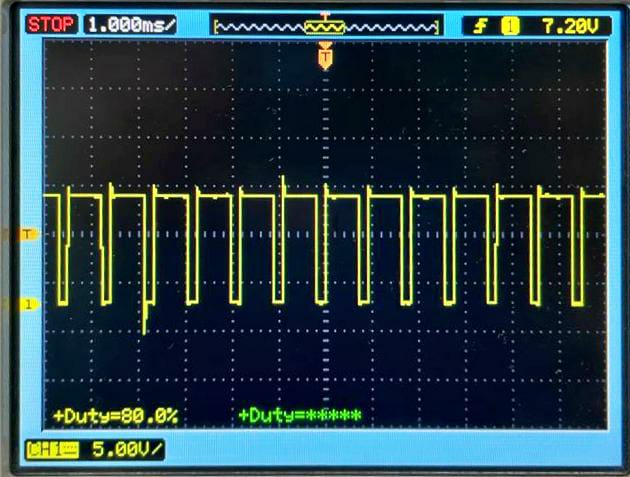
\includegraphics[width=0.9\columnwidth, height=110px]{WhatsApp Image 2022-06-22 at 5.49.02 PM (2).jpeg}} \\ \vspace{5px}
\end{center}
\end{multicols}
\vspace{5px}
\subsection{Power Circuit}
\begin{multicols}{2}
\begin{center}
\fcolorbox{black}{white}{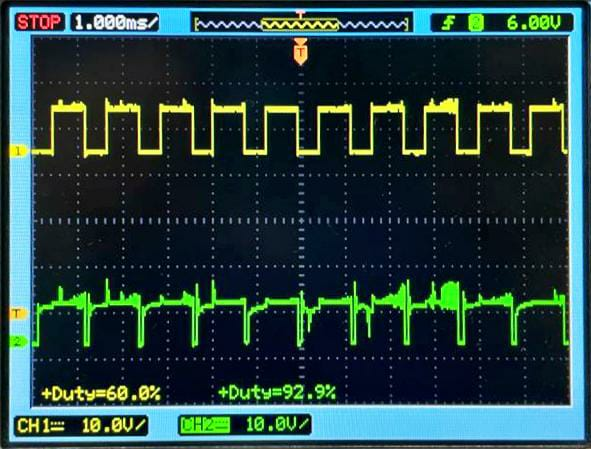
\includegraphics[width=0.9\columnwidth, height=110px]{WhatsApp Image 2022-06-22 at 5.49.02 PM.jpeg}} \\ \vspace{5px}

\columnbreak

\fcolorbox{black}{white}{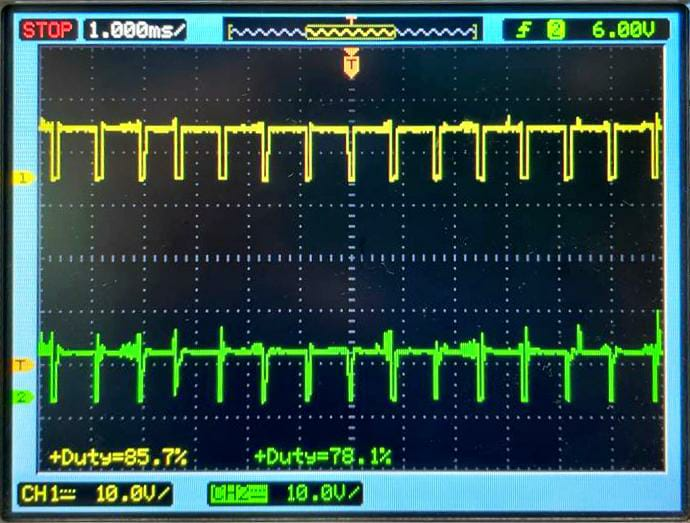
\includegraphics[width=0.9\columnwidth, height=110px]{WhatsApp Image 2022-06-22 at 5.49.03 PM.jpeg}} \\ \vspace{5px}
\end{center}
\end{multicols}


\section{Sources of Error}
\begin{itemize}
\item Scale of DSO not appropriate for measurements
\item Loose Connections
\item Resistance of wires not taken into account, and also giving rise to inconsistency due to increase in resistance due to heating
\item Change in the connections while circuit is closed.

\end{itemize}

\section{Precautions}

\begin{itemize}
\item Make the connections neat and tight
\item Don’t leave the switch on for long continuous periods of time.
\item Wear proper shoes and use insulated tools
\end{itemize}

\section{Concluding Remarks}
On the DSO, the output waveform for different values of $R_1$ and $R_2$ can be examined by connecting a potentiometer. We notice the following:
\begin{enumerate}
    \item The value of $R_1$ should not tend to $0 \ \Omega$. The circuit malfunctions if the value is close to $0 \ \Omega$. Thus, in ideal case, we should keep $R_1$ constant and vary $R_2$. Value of $R_1$ should be kept as low as $1k\Omega$ while $R_2$ should have a potentiometer of value $100k\Omega$.
    \item We verified that the waveform across the motor and output terminal of IC 555 Timer is same.
    \item When we decrease $R_2$, the speed of motor increases and when $R_2$ is $0 \ \Omega$, then motor runs at maximum speed.
    \item The Darlington transistor (TIP122) is a NPN Transistor. It acts as a switch in our case. When the output waveform is 0V, the transistor is in OFF State.
    \item A Freewheeling Diode is connected across the motor. When the Transistor is in OFF State, it helps the inductive load to freewheel the energy.
\end{enumerate}

\vspace{20px}

\section{Details of the Team Members}
\begin{enumerate}
    \item Aditya Agrawal 2021AM10198
    \item Yash Agarwal 2021EE10638
    \item Yogesh Yadav 2021CH10406
\end{enumerate}
\end{document}
